%%%%%%%%%%%%%%%%%%%%%%%%%%%%%%%%%%%%%%%%%%%%%%%%%%%%%%%%%%%%%%%%%%%%%%%%%%%%%%%%
%2345678901234567890123456789012345678901234567890123456789012345678901234567890
%        1         2         3         4         5         6         7         8
% DOCUMENT CLASS
\documentclass[oneside,12pt]{Classes/RoboticsLaTeX}

% USEFUL PACKAGES
% Commonly-used packages are included by default.
% Refer to section "Book - Useful packages" in the class file "Classes/RoboticsLaTeX.cls" for the complete list.
\usepackage{amsmath}
\usepackage{amsfonts}
\usepackage{multirow}
\usepackage{colortbl}
\usepackage{color}
\usepackage[table]{xcolor}
\usepackage{epigraph}
\usepackage{graphicx}
%\usepackage{subfigure}
\usepackage{caption}
\usepackage{subcaption}
\usepackage{hyperref}
\usepackage{tabularx}
\usepackage{float}
\usepackage{longtable}
\usepackage[pdftex]{graphicx}
\usepackage{pdfpages}
%\usepackage{tabularx}
\usepackage{pdflscape}
\usepackage[acronym,toc]{glossaries}
\usepackage{setspace}
\setstretch{1.5}
\usepackage{graphicx}
\usepackage{comment}
%\usepackage[toc,page]{appendix}
\usepackage{amsmath,amssymb}
\usepackage{mathrsfs}
\usepackage[english]{babel}
\usepackage[utf8]{inputenc}
\usepackage{algorithm}
%\usepackage{algorithmicx}
\usepackage{algcompatible}
\usepackage{xpatch}
\usepackage{tikz}
\usepackage{rotating}
\let\proof\relax
\let\endproof\relax
\usepackage{mathtools,amsthm}
\makeindex
\renewcommand{\algorithmiccomment}[1]{// #1}
\newtheorem{theorem}{Theorem}
\newtheorem{case}{Case}
\newtheorem{lemma}{Lemma}
\newtheorem{corollary}{Corollary}
\newtheoremstyle{case}{}{}{}{}{}{:}{ }{}
\theoremstyle{case}
\usetikzlibrary{shapes,snakes,decorations.pathmorphing}
\tikzset{node distance=2.5cm, every edge/.style={draw,
		->,thick},snake it/.style={decorate, decoration=snake}}
\tikzstyle{player1}=[circle,draw=black!100,fill=white!20,thick,inner sep=0pt,minimum size=8mm]
\tikzstyle{safeReach}=[circle,draw=white!100,fill=white!20,thick,inner sep=0pt,minimum size=8mm]
\tikzstyle{player2}=[rectangle,draw=black!100,fill=white!20,thick,inner sep=0pt,minimum size=7mm]
\tikzstyle{otherLabel}=[circle,draw=black!100,fill=white!20,thick,inner sep=0pt,minimum size=20mm]
\tikzstyle{cpreLabel}=[rectangle,draw=black!100,fill=white!20,thick,inner sep=0pt,minimum size=40mm]
% Various Environments
\newcommand{\be}{\begin{enumerate}}
	\newcommand{\ee}{\end{enumerate}}
\newcommand{\bi}{\begin{itemize}}
	\newcommand{\ei}{\end{itemize}}


% Special characters
\newcommand{\cL}{\mbox{{$\cal L$}}}
\newcommand{\cN}{\mbox{{$\cal N$}}}
\newcommand{\cQ}{\mbox{{$\cal Q$}}}
\newcommand{\cR}{\mbox{{$\cal R$}}}
\newcommand{\cF}{\mbox{{$\cal F$}}}
\newcommand{\cM}{\mbox{{$\cal M$}}}
\newcommand{\cS}{\mbox{{$\cal S$}}}

% Abbreviations
\newcommand\eg{\textit{e.g.}}
\newcommand\etc{\textit{etc.}}
\newcommand\etal{\textit{et al.}}
\newcommand\ie{\textit{i.e.}}
\newcommand\cf{\textit{cf.}}

% mathematical abbreviations
\newcommand{\ra}{\rightarrow}
\newcommand{\Ra}{\Rightarrow}
\newcommand{\ua}{\uparrow}
\newcommand{\La}{\Leftarrow}
\newcommand{\Lra}{\Leftrightarrow}
\newcommand{\lra}{\longrightarrow}
\newcommand{\rhp}{\rightharpoonup}
%\onehalfspacing
% SPECIAL COMMANDS
% correct bad hyphenation
\hyphenation{op-tical net-works semi-conduc-tor}
\hyphenation{par-ti-cu-lar mo-du-le ge-stu-re}
% INTERLINEA 1.5
%\renewcommand{\baselinestretch}{1.5}

%% ignore slightly overfull and underfull boxes
%\hbadness=10000
%\hfuzz=50pt
% declare commonly used operators
\DeclareMathOperator*{\argmax}{argmax}

% HEADER
%\ifpdf
   % \pdfinfo {/Title (Example of PhD Thesis with RoboticsLaTeX template)
    %          /Creator (TeX)
     %         /Producer (pdfTeX)
      %        /Author (Barbara Bruno, Fulvio Mastrogiovanni)
       %       /CreationDate (D:20141024182500) %format D:YYYYMMDDhhmmss
        %      /ModDate (20141024182500)
         %     /Subject (Example of PhD Thesis with RoboticsLaTeX template)
          %    /Keywords (PhD, Thesis, Example, RoboticsLaTeX)}
%    \pdfcatalog {/PageMode (/UseOutlines)
%                 /OpenAction (fitbh) }
%\fi

\title{\Large{Admissible Strategies for Safety and Reachability Objectives in Graph Games}}

\ifpdf
  \author{Prasita Mukherjee \\ { (174101042)}
          }
  \collegeordept{Department of Computer Science and Engineering}
  \university{Indian Institute of Technology Guwahati}
  \crest{
\includegraphics[bb = 0 0 292 336, width=40mm]{iitg}}
\else
  \author{Prasita Mukherjee \newline (174101042)
          }
  \collegeordept{Department of Computer Science and Engineering}
  \university{Indian Institute of Technology Guwahati}
  \crest{
\includegraphics[bb = 0 0 292 336, width=40mm]{iitg}}
\fi
 %nome relatore tesi 
\supervisor{Dr. Purandar Bhaduri}

% DECLARATION
 %Use the following command to change the declaration text:

\degree{Master of Technology, Computer Science and Engineering}
\degreedate{May 16, 2019}

%%%%%%%%%%%%%%%%%%%%%%%%%%%%%%%%%%%%%%%%%%%%%%%%%%%%%%%%%%%%%%%%%%%%%%%%%%%%%%%%
%\makeglossaries
%\loadglsentries{glossary}
\begin{document}

% A page with the abstract and running title and author etc may be
% required to be handed in separately. If this is not so, comment
% the following 3 lines:
% \begin{abstractseparate}
%   %%%%%%%%%%%%%%%%%%%%%%%%%%%%%%%%%%%%%%%%%%%%%%%%%%%%%%%%%%%%%%%%%%%%%%%%%%%%%%%%
%2345678901234567890123456789012345678901234567890123456789012345678901234567890
%        1         2         3         4         5         6         7         8
% THESIS ABSTRACT

% Use the following style if the abstract is long:
%\begin{abstractslong}
%\end{abstractslong}

\begin{abstracts}

Finding winning strategies for \textit{Player~1} (the system) against \textit{Player~2} (the environment) in graph games is the basis for synthesizing controllers satisfying a specification. In many situations where winning strategies do not exist, it is important to compute the best-effort (or admissible) strategies. The thesis aims to compute admissible strategies for safety and reachability objectives in graph games. 

\end{abstracts}

% \end{abstractseparate}
\begin{spacing}{1}
\maketitle
\end{spacing}

% add an empty page after title page
\newpage\null\thispagestyle{empty}\newpage

% set the number of sectioning levels that get number and appear in the contents
\setcounter{secnumdepth}{3}
\setcounter{tocdepth}{3}


\frontmatter
%%%%%%%%%%%%%%%%%%%%%%%%%%%%%%%%%%%%%%%%%%%%%%%%%%%%%%%%%%%%%%%%%%%%%%%%%%%%%%%%
%2345678901234567890123456789012345678901234567890123456789012345678901234567890
%        1         2         3         4         5         6         7         8
% THESIS ACKNOWLEDGEMENTS

% Use the following style if the acknowledgements are long:
%\begin{acknowledgementslong}
%\end{acknowledgmentslong}

\begin{acknowledgements}


%“I don't know half of you half as well as I should like; and I like less than half of you half as well as you deserve.”
 %J.R.R. Tolkien, The Fellowship of the Ring 

I express my sincere gratitude towards my guide \textbf{Dr. Purandar Bhaduri} for his constant support, encouragement and inspiration throughout the project work. I specially acknowledge him for his advice, supervision, and the vital contribution as and when required. It is because of his constant and general interest and assistance that this project has been successful. 

I want to acknowledge my parents for motivating me and providing moral support during the course time of M.Tech. I also want to acknowledge the Department Of Computer Science  and inter department teaching members for helping me by giving the basic idea.


\end{acknowledgements}

\begin {Certificate}
\begin{large}
This is to certify that the project work entitled \textbf{Admissible Strategies for Safety and Reachability Objectives in Graph Games} being submitted to Department of Computer Science and Engineering, Indian Institute of Technology Guwahati by \textbf{Prasita Mukherjee}, in partial fulfillment for the award of the degree of Master of Technology, Computer Science and Engineering in, is a bonafide work carried out by her under my supervision. To the best of my knowledge it has not been submitted elsewhere for award of degree.
\end{large}
\\[4cm]
\begin{flushright}

........................\par
\textbf{Dr. Purandar Bhaduri}\\
Professor\\
Department of Computer Science and Engineering\\
Indian Institute of Technology Guwahati\\

\normalfont
\end{flushright}
\end {Certificate}
%%%%%%%%%%%%%%%%%%%%%%%%%%%%%%%%%%%%%%%%%%%%%%%%%%%%%%%%%%%%%%%%%%%%%%%%%%%%%%%%
%2345678901234567890123456789012345678901234567890123456789012345678901234567890
%        1         2         3         4         5         6         7         8
% THESIS ABSTRACT

% Use the following style if the abstract is long:
%\begin{abstractslong}
%\end{abstractslong}

\begin{abstracts}

Finding winning strategies for \textit{Player~1} (the system) against \textit{Player~2} (the environment) in graph games is the basis for synthesizing controllers satisfying a specification. In many situations where winning strategies do not exist, it is important to compute the best-effort (or admissible) strategies. The thesis aims to compute admissible strategies for safety and reachability objectives in graph games. 

\end{abstracts}


\tableofcontents
\listoffigures
%\listoftables
%\printglossary[title=List of Acronyms,type=\acronymtype]
%\printglossary  % Print the nomenclature (WAY TOO COMPLEX FOR ME NOW!)
%\addcontentsline{toc}{chapter}{Nomenclature}

\mainmatter
%%% Thesis Introduction --------------------------------------------------
\chapter{Introduction}
\label{Sec:Introduction}
Games played on finite graphs, typically involving two players, have
been a subject of widespread investigation in the field of computer
science, with applications primarily in the field of controller
synthesis~\cite{SynthesisOfReactiveModule}. Typically, a winning
strategy for \textit{Player~1} (the system) against \textit{Player~2}
(the environment) gives rise to a controller that satisfies a given
specification.

The games considered have a set of winning and losing nodes for
\textit{Player~1}. In this work, the primary focus is on losing nodes
and attempt to achieve \textit{best-effort strategies}, also known as
\textit{admissible strategies}~\cite{OmegaRegularGames}. In many
applications finding such a best-effort strategy when a winning
strategy does not exist from a given node is very useful. Instances of
such applications are problems which do not involve a strong sense of
competition, \ie, \textit{Player~2} can be cooperative rather than
adversarial or more realistically when \textit{Player~2} is rational,
\ie, focused more on achieving its own objective rather than thwarting
\textit{Player~1} from meeting its goal. This happens, for instance,
in component-based systems where the components are autonomous agents
such as robots which have their own objectives to meet and are not
necessarily adversarial. In such cases, \textit{Player~1} can end up
winning if this does not prevent \textit{Player~2} from meeting its
goal, even if there is no strategy that will win against all
\textit{Player~2} strategies.

\textit{Safety} and \textit{reachability} are two very important goals
in system design. Safety requires plays to remain forever within a
safe set of nodes, whereas reachability requires a set of nodes to be
visited after finitely many steps. The work computes admissible
strategies for these two types of objectives.

Admissible strategies are also known as \textit{non-dominated
	strategies} \ie, the game can be lost by such strategies if and only
if no other strategy can win the game starting from the same node
against any strategy of \textit{Player~2}. In this work, the
perspective of \textit{Player~1} is taken into consideration. The semantics are defined
analogously when played from \textit{Player~2's} perspective and the
algorithms hold good. The notion of \textit{admissibility} is slightly
different from Faella~\cite{AdmissibleInfiniteGames} and is consistent
with the definition of Brenguier \etal~\cite{OmegaRegularGames}.

The rest of the thesis is organized as follows. First the
related work done in this area is discussed in Chapter~\ref{Sec:RelatedWork},
followed by the preliminaries and definitions
in \ref{Sec:Preliminaries}. Then the two algorithms
developed for safety and reachability objectives are discussed in
Chapters~\ref{Sec:Safety} and \ref{Sec:Reachability} respectively,
along with their time complexity.
\chapter{Related Work}
\label{Sec:RelatedWork}
Determining the winning set of nodes and the winning strategies in a
graph game had been a primary concern in the past, and significant
work has been done for safety, reachability and more general
$\omega$-regular objectives in this
area~\cite{AutomataLogicsInfiniteGames}. Work on cooperation and
rational behavior of players is now an emergent area of
research~\cite{AssumptionSynthesis,PerimeterOfWorldModel,CompositionalSynthesis,AdmissibleInfiniteGames,RationalSynthesis}.

Faella~\cite{AdmissibleInfiniteGames} discussed the potential benefits
of real world applications in playing a game from a \textit{losing}
node in a rational way to achieve the best possible results. His
primary focus was on \textit{best-effort strategies} by relying on the
cooperation of the other player. He outlined a procedure to compute
admissible strategies for \emph{positional} and
\textit{prefix-independent} goals, where the latter are goals closed
under adding or deleting finite prefixes to/from its elements. But he
did not provide a method for goals which are not prefix-independent,
such as safety and reachability. He claimed that if all \textit{Player
	2} nodes are treated as \textit{Player~1} nodes, then the winning
strategies obtained, called \emph{cooperatively winning}, are also
admissible for safety and reachability objectives. It is shown via
examples that this claim is incorrect and algorithms are provided for
finding admissible strategies for safety and reachability objectives,
arguably the most important among all goals which are
non-prefix-independent.

Bloem \etal~\cite{AssumptionSynthesis} discussed various approaches
for dealing with assumptions on environment behavior while solving
games. They proposed four goals which should be met by all system
designs, out of which what is relevant here is the goal of ``not
giving up'' when the system guarantee cannot be enforced under
worst-case assumptions. As mentioned above, in many situations, the
environment may not be perfectly adversarial and provide the
worst-case input. In such cases, it makes sense for the system to try
to meet its goal as much as possible, assuming some level of
cooperation from the environment. The work addresses precisely this
situation, finding admissible strategies for the important cases of
safety and reachability objectives. Note that, by definition,
admissible strategies make the minimal assumptions about cooperation
from the other player.

Damm and
Finkbeiner~\cite{PerimeterOfWorldModel,CompositionalSynthesis}
proposed algorithms for synthesizing and verifying dominant strategies
which is based on construction of tree automata for objectives
specified in LTL.  The notion of dominant strategy considered in the
work is identical to what is called an admissible strategy in this
work. The work is a special case of
\cite{PerimeterOfWorldModel,CompositionalSynthesis}, which considers
safety and reachability objectives. The algorithms developed are also much
simpler, based primarily on graph-theoretic notions and of lower
complexity than the double exponential algorithm in
\cite{PerimeterOfWorldModel,CompositionalSynthesis}.


In \cite{RationalSynthesis}, Fisman \etal\ introduce the idea of
rational synthesis, \ie, synthesis in the context of multiple
autonomous agents where each agent has a goal of its own and the goals
are not necessarily adversarial. The approach provides a strategy not
just for the agent in question (called the \emph{system agent} in
\cite{RationalSynthesis}) but for all the agents such that the
specification of the system agent is satisfied and the strategy
profile for all the agents meet some desired solution concept, such as
the existence of a dominant strategy, Nash equilibrium, or
subgame-perfect equilibrium. In such equilibria, no agent has the
incentive to unilaterally deviate from its strategy. While admissible
strategies are clearly related to the problem of rational synthesis,
exploring the exact relationship is part of future work.

\chapter{Preliminaries}
\label{Sec:Preliminaries}
A \textit{game structure} \textit{G} is defined as a pair $(V, E)$ where
\begin{enumerate}
	\item $V = V_{1} \uplus V_{2}$ represents the finite set of vertices/nodes in the game graph, where $V_{1}$ and $V_{2}$ are the sets of \textit{Player~1} and \textit{Player~2} nodes respectively.
	\item $E\subseteq V \times V$ represents the finite set of edges in the game graph. Every node in V has a successor, \ie, $\forall v \in V, \exists v' \in V . (v,v') \in E$.
\end{enumerate}

A \textit{play} in $G$ is defined as a sequence of nodes $v_{0} v_{1}
v_{2} \ldots$ such that $(v_{i},v_{i+1}) \in E$. If the current node
$v \in V_{1}$, then \textit{Player~1} makes the next move by selecting
an edge $(v,v') \in E$ that takes the game to $v'$. If the current
node $v \in V_{2}$, a \textit{Player~2} move is defined analogously. A
\textit{game} $\mathcal{G} = (G,\mathit{Win})$ is a pair of a game structure
and a winning condition $\mathit{Win}$, given by a set of plays in $G$.

A game can have various winning conditions (like
\textit{B$\ddot{u}chi$}, \textit{Muller}, \textit{Parity}, etc.) that
specify the set $\mathit{\mathit{Win}}$ of plays that are won by
\textit{Player~1}. In the work, only safety and
reachability objectives are considered. For a game structure $G = (V,E)$, a
\textit{safety objective} is given by a set $S \subseteq V$ of
nodes. A play $v_{0}v_{1}v_{2}\ldots$ in $V^{\omega}$ is safe,
\ie, winning for \textit{Player~1}, if it never leaves the set $S$,
\ie, $v_{i} \in S$ for all i$\in \mathbb{N}$. \textit{Player~1} loses
the game if the play enters V$\backslash$S at any point.  A
\textit{reachability objective} is specified by a set $R \subseteq V$
of nodes. The goal for \textit{Player~1} is to force the game to reach
a node in $R$, \ie, a play $v_{0}v_{1}v_{2}\ldots$ is winning
for \textit{Player~1} if $v_{i} \in R$ for some i$\in \mathbb{N}$.

A \textit{strategy} for \textit{Player~1} is defined by a function $
\sigma : V^{*}V_{1} \rightarrow V $ that maps the history of observed
nodes to the next node. A \textit{Player~2} strategy is defined
analogously. Given strategies $\sigma$ and $\rho$ for \textit{Player
	1} and \textit{Player~2} respectively, the work defines \textit{Out}($
\sigma, \rho, v$) as the unique word $v_{0} v_{1} v_{2}..$ in
$V^{\omega}$ such that $v_{i+1} = \sigma(v_{i})$ if $v_{i} \in V_{1}$
and $v_{i+1} = \rho(v_{i})$ otherwise, for all $i \in \mathbb{N}$ and
$v_{0} = v$. The work defines \textit{Out}($\sigma,v$) = \{\textit{Out}($
\sigma, \rho, v) \: | \: \rho$ is a \textit{Player~2} strategy\} as
the set of outcomes from node $v$ when \textit{Player~1} plays
according to strategy $\sigma$. A strategy $\sigma$ for \textit{Player
	1} from node $v$ is \textit{winning} if \textit{Out}($\sigma,v)
\subseteq \mathit{\mathit{Win}}$, where $\mathit{\mathit{Win}}$ is a set of winning
plays, \ie, $\sigma$ is a winning strategy for \textit{Player~1} if
for all \textit{Player~2} strategies $\rho$, \textit{Out}($ \sigma,
\rho, v) \in$ $\mathit{\mathit{Win}}$. The work defines $val(\sigma,\rho,v)$ as 1 if
$Out(\sigma, \rho, v) \in \mathit{\mathit{Win}}$ and 0 otherwise.  For a game
$\mathcal{G}$, a strategy for $\sigma$ for \textit{Player~1} is said
to be \textit{positional} (or \textit{memoryless}) if $\sigma$ depends
only on the last node of the current history of the game \ie, there
is a function $f\: : V_{1} \rightarrow V $ such that
$\sigma(sv_{1})\:= \:f(v_{1})$ for all $s \in V^{*}$. For the winning
conditions of safety and reachability, positional strategies suffice
and hence attention is restricted to such strategies in the rest of the thesis.

The following definitions appear in \cite{OmegaRegularGames}. For any two \textit{Player~1} strategies $\sigma_{1}$ and $\sigma_{2}$, $\sigma_{1}$ \textit{very weakly dominates} $\sigma_{2}$ at node $v$, if $val(\sigma_{1}, \rho, v) \geq val(\sigma_{2}, \rho, v)$.
A \textit{Player~1} strategy $\sigma_{1}$ is \textit{dominated} by another \textit{Player~1} strategy $\sigma_{2}$ at node $v$, if $val(\sigma_{1}, \rho, v) \leq val( \sigma_{2}, \rho, v)$, for all \textit{Player~2} strategies $\rho$ and $val(\sigma_{1}, \rho, v) < val(\sigma_{2}, \rho, v)$ for at least one \textit{Player~2} strategy $\rho$. It is also said $\sigma_{2}$ \textit{dominates} $\sigma_{1}$ at $v$ in such a case.
An \textit{admissible strategy} for \textit{Player~1} is a strategy $\sigma_{1}$ that is not dominated by any other \textit{Player~1} strategy $\sigma_{2}$ at any vertex $v$. 
\begin{figure}[thpb]
	\centering
	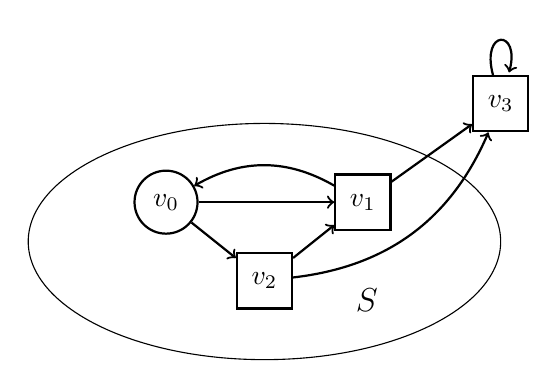
\begin{tikzpicture}
	\draw (0,0) ellipse (3cm and 1.5cm);
	\node at (1.3,-0.75) [safeReach] {\large $S$};
	\node at (0,-0.5) [player2] (1) {$v_{2}$};
	\node at (1.25,0.5) [player2] (2) {$v_{1}$};
	\node at (-1.25,0.5) [player1] (3) {$v_{0}$};
	\node at (3,1.75) [player2] (4) {$v_{3}$};
	\draw (4) edge[loop above] (4);
	\draw (3) edge (2);
	\draw (3) edge (1);
	\draw (1) edge (2);
	\draw (2) edge[bend right] (3);
	\draw (2) edge (4);
	\draw (1) edge[bend right] (4);
	\end{tikzpicture}
	\caption{Admissible strategy for safety}
	\label{figurelabel7}
\end{figure}
\begin{figure}[thpb]
	\centering
	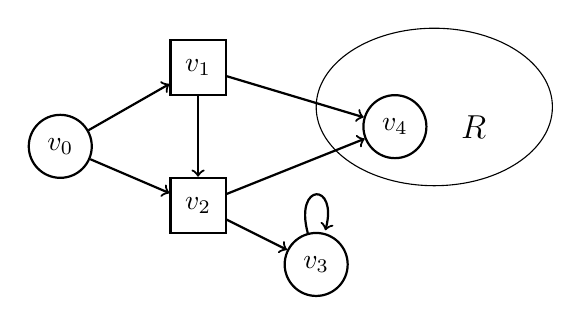
\begin{tikzpicture}
	\draw (3,1) ellipse (1.5cm and 1cm);
	\node at (3.5,0.75) [safeReach] {\large $R$};
	\node at (0,-0.25) [player2] (1) {$v_{2}$};
	\node at (0,1.5) [player2] (2) {$v_{1}$};
	\node at (-1.75,0.5) [player1] (3) {$v_{0}$};
	\node at (1.5,-1) [player1] (4) {$v_{3}$};
	\node at (2.5,0.75) [player1] (5) {$v_{4}$};
	\draw (4) edge[loop above] (4);
	\draw (3) edge (2);
	\draw (3) edge (1);
	\draw (2) edge (1);
	\draw (1) edge (4);
	\draw (1) edge (5);
	\draw (2) edge (5);
	\end{tikzpicture}
	\caption{Admissible strategy for reachability}
	\label{figurelabel8}
\end{figure}

Figures~\ref{figurelabel7} and \ref{figurelabel8} depict examples of
admissible strategies for safety and reachability, when there does not
exist a winning strategy for \textit{Player~1} from node
$v_{0}$. Throughout the thesis \textit{Player~1} nodes are depicted by
circles and \textit{Player~2} nodes by squares.
Figure~\ref{figurelabel7} is an example of a game with a safety
objective, where $S = \{v_{0},v_{1},v_{2}\}$. Here \textit{Player~1}
does not have a winning strategy from $v_{0}$ as \textit{Player~2} can
always take the game to $v_{3}$. But the \textit{Player~1} strategy
$\sigma_{1}$, which chooses the edge ($v_{0}$,$v_{1}$) is better than
the strategy $\sigma_{2}$, which chooses the edge ($v_{0}$,$v_{2}$),
because the former performs strictly better than the latter against
the \textit{Player~2} strategy \{$v_{1} \mapsto v_{0}, v_{2} \mapsto
v_{3}, v_{3} \mapsto v_{3}$\}. Similarly for the reachability game
depicted in Figure~\ref{figurelabel8} with $R=\{v_4\}$, there does not
exist a winning strategy for \textit{Player~1} from $v_{0}$. But the
\textit{Player~1} strategy $\sigma_{1}$ which chooses the edge
$(v_{0},v_{1})$ is better than the strategy $\sigma_{2}$ which chooses
the edge $(v_{0},v_{2})$, because the former performs strictly better
than the latter against the \textit{Player~2} strategy \{$v_{1}
\mapsto v_{4}, v_{2} \mapsto v_{3}$\}. These two examples also show
that treating all \textit{Player~2} nodes as \textit{Player~1} nodes
and finding winning strategies for \textit{Player~1} does not identify
the admissible strategies for safety and reachability games as claimed
by Faella~\cite{AdmissibleInfiniteGames}.
\chapter{Admissible Strategies for Safety Games}
\label{Sec:Safety}
In this chapter, the algorithm is described for finding admissible
strategies for safety games and proof for its correctness is provided.  Here the
controllable predecessor operator $\mathit{CPre}(T)$ for $T \subseteq
V$ determines the set of nodes from which \textit{Player~1} can force
the game to move to a node in $T$ in one step:
$\mathit{CPre}(T) = \{u | u \in V_{1} \: and \: \exists v \in T, (u,v) \in E \}\cup \{u | u \in V_{2} \: and \: \forall v, (u,v) \in E \Rightarrow v \in T\}$.

Algorithm~\ref{alg:algorithm1} presented below computes the
set of winning nodes for safety games specified by a safe set $S$,
while playing from the perspective of \textit{Player~1}. It computes
the winning nodes by computing the greatest fixed point of a monotone
operator on $(2^{V}, \subseteq)$~\cite{SynthesisInfiniteGames}.

\begin{algorithm}
	\caption{Winning Nodes for Safety Games}
	\textbf{Input} Game structure $G := (V,E)$ and $S \subseteq V$, the set of safe nodes \\ 
	\textbf{Output} Set of winning nodes $W$
	\label{alg:algorithm1}
	\begin{algorithmic}[1]
		\STATE \textit{T} := S
		\STATE $Y_{0}$ := \textit{T}
		\STATE i := 1
		\STATE $Y_{i}$ := $\textit{T} \cap \mathit{CPre}(Y_{i-1})$
		\STATE if $Y_{i} \neq Y_{i-1}$ then i := i + 1. Goto step 4
		\STATE $W$ := $Y_{i}$
		\STATE \textbf{return} $W$
	\end{algorithmic}
\end{algorithm}



Before presenting the algorithm for computing admissible strategies
for safety games (Algorithm~\ref{alg:algorithm2}), a few
definitions are needed. These definitions apply to the subgraph $G' := (S,E')$ of
$G$ induced by the safe set $S$ of nodes, since for nodes in $V
\backslash S$ all strategies are losing for \textit{Player~1}.

A \textit{potentially winning node} is a \textit{Player~2} node not in
$W$ (\ie, it is a losing node for \textit{Player~1}) which lies on a
cycle contained in the safe set $S$. A \textit{safety-admissible
	cycle} (s-admissible cycle in brief) is a cycle that lies within $S$
and contains at least one potentially winning node and does not
contain a node in $W$. An s-admissible cycle $C$ with a set of
potentially winning nodes $H$ is \textit{minimal} if there is no other
s-admissible cycle $C'$ with the set of potentially winning nodes $H'$
such that $H'$ is strictly contained in $H$. \textit{Paths}($u$,$v$)
is the set of paths from $u$ to $v$ in the subgraph $G'$ of $G$
induced by $S$. Minimal s-admissible cycles play a crucial role in
identifying all admissible strategies for safety games. At any
\textit{Player~1} node $v$ in a minimal s-admissible cycle $C$, if
\textit{Player~1} chooses its successor in $C$ as the next node, then
this gives rise to an admissible strategy. Also, for a \textit{Player
	1} node $v$ in $S \backslash W$, which is not in an s-admissible
cycle, the work defines a \textit{minimal safety-admissible path} (minimal
s-admissible path in brief) from $v$ as a path $P$ from $v$ in $S$
leading either to a minimal s-admissible cycle or to a node in $W$
satisfying the following minimality condition: for no other path $Q$
from $v$ leading either to a minimal s-admissible cycle or to a node
in $W$ is the set of potentially winning nodes on $Q$ a proper subset
of the corresponding set on $P$. At any \textit{Player~1} node $v$ on a
minimal s-admissible path $P$, if \textit{Player~1} chooses its
successor in $P$ as the next node, then this also gives rise to an
admissible strategy. The work claims that identifying all minimal
s-admissible cycles and minimal s-admissible paths is necessary and
sufficient for identifying all admissible strategies. This claim is
proved in Theorem~\ref{theorem1} below.

Algorithm~\ref{alg:algorithm2} is presented, which computes
the set of admissible strategies for safety games. In step 1, the winning set of nodes $W$ for \textit{Player~1} is computed using
Algorithm~\ref{alg:algorithm1}. In step 2, the subgraph
$G'$ of $G$ induced by $S$ is constructed. For every node $v$ that is in $(V_{1} \cap
S) \backslash W$, Algorithm~\ref{alg:algorithm3} is executed to determine the set of admissible strategies. In steps 5,6 and 7 the work outputs the set of all admissible strategies for \textit{Player~1}
nodes. If a node is winning, \textit{Player~1} can play according to
any winning strategy. If a node is not in $S$, \textit{Player~1} can
play arbitrarily. For the remaining nodes, \textit{Player~1} plays
according to the strategies obtained from Algorithm~\ref{alg:algorithm3}.

\begin{algorithm}
	\caption{Admissible Strategies for Safety Games}
	\textbf{Input} Game structure $G := (V,E)$ and $S \subseteq V$, the set of safe nodes \\ 
	\textbf{Output} Set of admissible strategies for \textit{Player~1} nodes
	\label{alg:algorithm2}
	\begin{algorithmic}[1]
		\STATE Compute the set of winning nodes $W$ for \textit{Player~1} using Algorithm~\ref{alg:algorithm1}
		\STATE Construct subgraph $G' := (S,E')$ of $G$ induced by $S$
		\STATE Mark every $v \in (V_{1} \cap S) \backslash W$ as not visited
		\STATE For every node in step 3 which is not visited, execute Algorithm~\ref{alg:algorithm3} on $v$
		\STATE At any \textit{Player~1} node $v \in W$, play according to any winning strategy
		\STATE At any \textit{Player~1} node $v \notin S$, choose an arbitrary move
		\STATE At any remaining \textit{Player~1} node $v \in S$, play according to strategies returned for $v$ in Algorithm~\ref{alg:algorithm3}
	\end{algorithmic}
\end{algorithm}

Algorithm~\ref{alg:algorithm3} presented below computes the values of
all admissible strategies for a \textit{Player~1} node $v$,
considering the induced subgraph $G' := (S,E')$. For each such node
$v$ set $PW(v)$ is maintained, each element of which is a pair
consisting of one of the following:
\begin{enumerate} 
	\item a set of potentially winning \textit{Player~2} nodes on an s-admissible path from $v$ to a set in $W$ and $v'$ the successor of $v$ on such a path, or
	\item a set of potentially winning \textit{Player~2} nodes on an s-admissible cycle containing $v$, and $v'$ the successor of $v$ on such a cycle, or
	\item a set of potentially winning \textit{Player~2} nodes on a path from $v$ which is an s-admissible path followed by an s-admissible cycle (also called a \textit{safety-admissible lasso} (s-admissible lasso in brief)) and $v'$ the successor of $v$ on such a lasso.
\end{enumerate}
The algorithm explores every path starting from $v$.  Whenever one of the following happens, update $PW(v)$: 
\begin{enumerate} 
	\item a node $u \in W$ is encountered, or
	\item an s-admissible cycle containing $v$ is found or,
	\item an s-admissible path leading to an s-admissible cycle is found.
\end{enumerate} 
Admissible strategies are determined by finding the minimal sets $MinPW(v)$ in $PW(v)$, \ie, ones that are not strictly contained in any other set, for each successor $v'$ of $v$. Then an admissible strategy will always choose an edge $(v,v')$ which lies on a path containing the set of potentially winning nodes $v$ such that $(v,v') \in MinPW(v)$.

\begin{algorithm}
	\caption{Values of admissible strategies at $v \in (V_{1} \cap S) \backslash W$}
	\textbf{Input} $v\in V_{1}$ \\ 
	\textbf{Output} Values of all admissible strategies for $v$
	\label{alg:algorithm3}
	\begin{algorithmic}[1]
		\STATE Mark $v$ as visited
		\STATE Initialize $PW(v) \: := \: \emptyset$
		\STATE Explore every path from $v$ and update $PW(v)$ when one of the following happens:
		\begin{case}
			A node $u \in W$, the winning set of nodes is encountered
			\newline $PW(v) := PW(v) \cup (\{ X | X$ is the set of all \textit{Player~2} nodes on the path from $v$ to $u\in W\},v')$, where $v'$ is the successor of $v$ on the path    
		\end{case}
		\begin{case}
			An s-admissible cycle containing $v$ is found
			\newline $PW(v) := PW(v) \cup (\{ X | X$ is the set of all \textit{Player~2} nodes on the s-admissible cycle containing $v\},v')$, where $v'$ is the successor of $v$ on the s-admissible cycle
		\end{case}
		\begin{case}
			An s-admissible lasso is found
			\newline $PW(v) := PW(v) \cup (\{ X | X$ is the set of all \textit{Player~2} nodes on the s-admissible lasso$\},v')$, where $v'$ is the successor of $v$ on the s-admissible lasso
		\end{case}
		\STATE Determine all minimal s-admissible paths and cycles by comparing the sets in $PW(v)$ for each $v'$ with respect to containment and store them in $MinPW(v)$
		\STATE Store the $(v,v')$ obtained in step 4 in the set $Next(v)$
		\STATE If $Next(v) \neq \emptyset$ then, \textbf{return} each element of $Next(v)$ as values of admissible strategies at $v$
		\STATE else \textbf{return} all pairs $(v,v') \in E$ as values of admissible strategies at $v$
	\end{algorithmic}
\end{algorithm}
\begin{theorem}
	\label{theorem1}
	The following statements are equivalent:
	\begin{enumerate}
		\item $\sigma$ is an admissible \textit{Player~1} strategy
		\item $\sigma(v) = v'$, where $v$ is a \textit{Player~1} node
		satisfying one of the following conditions:
		\newline (i) $v \in S \backslash W$ and $v$ lies on a minimal s-admissible cycle, or $v$ lies on a minimal s-admissible lasso or there is a minimal s-admissible path from $v$ to a node in $W$, and $v'$ is the successor of $v$ on such a cycle or lasso or path, or
		\newline (ii) $v \in W$ and $\sigma^{'}(v) = v'$ for some winning strategy $\sigma^{'}$, or
		\newline (iii) $v$ is any other node, \ie, $v \notin S$, and $\sigma(v)$ is any successor of $v$ in $G$
	\end{enumerate}
\end{theorem}
\begin{proof}
	$\mathit{1} \Rightarrow \mathit{2}$
	\newline Suppose $\sigma$ is an admissible \textit{Player~1} strategy such that for some \textit{Player~1} node $v \in S \backslash W$ $\sigma(v) = v'$ is not the successor of $v$ in a minimal s-admissible cycle, a minimal s-admissible path or a minimal s-admissible lasso. Clearly $v'$ must either be on an s-admissible path or on an s-admissible cycle or lasso, since otherwise even \textit{Player~2's} cooperation cannot ensure that the resulting play is in $S$. Suppose $v'$ is on an s-admissible cycle $C'$, which has the set of potentially winning nodes $H'$ which is not minimal, and hence by assumption there is a successor $v''$ of $v$ on an s-admissible path leading to a node in $W$, cycle or lasso with the potentially winning node set being $H"$, such that $H"$ is strictly contained inside $H'$. Let $u \in H' \backslash H"$. Then $val(\sigma,\rho,v) < val(\sigma',\rho,v)$, where $\sigma$ is identical to $\sigma'$ at all nodes except at node $v$ where $\sigma'(v) = v''$ and the \textit{Player~2} strategy $\rho$ plays according to the winning strategy for \textit{Player~2} at $u$ \ie, it takes the game outside $S$ (which exists by definition of a potentially winning node) and cooperates at every other node, \ie, chooses a successor node in the s-admissible cycle. This is a contradiction. The case for $v'$ being on an s-admissible path or lasso is similar. 
	\newline $\mathit{2} \Rightarrow \mathit{1}$
	\newline Suppose $\sigma$ is a \textit{Player~1} strategy satisfying the following: for $v \in S \backslash W$ lying on an s-admissible path or cycle $\sigma(v) = v'$, where $v'$ is the successor of $v$ in a minimal s-admissible cycle; for $v \in W$, $\sigma$ plays according to any winning strategy, and for any other $v$ plays arbitrarily. Suppose $\sigma$ is not admissible, \ie, it is dominated by a \textit{Player~1} strategy $\sigma'$. Clearly for nodes in $W$ and nodes in $S \backslash W$ from which there is no s-admissible paths, cycles or lassos, $\sigma'$ cannot be better than $\sigma$. Suppose $val(\sigma,\rho,v) < val(\sigma',\rho,v)$ at some node $v$, where $v$ lies on an s-admissible cycle, path or lasso. This implies that $Out(\sigma,\rho,v) \notin \mathit{Win}$ but $Out(\sigma',\rho,v) \in \mathit{Win}$.
	Then $Out(\sigma',\rho,v)$ must be an s-admissible cycle, s-admissible lasso or contain an s-admissible path leading to a winning node. By assumption $\sigma(v) = v'$ for $v \in S \backslash W$ lying on a minimal s-admissible path or cycle where $v'$ is the successor of $v$ on such a path, cycle or lasso. This means that there is a potentially winning \textit{Player~2} node $u$ on an s-admissible path, lasso or cycle from $v$ which occurs on $Out(\sigma',\rho,v)$ but not on $Out(\sigma,\rho,v)$. This implies there is a \textit{Player~2} strategy $\rho$ (in which \textit{Player~2} cooperates at every potentially winning node on $Out(\sigma,\rho,v$) but not at $u$) where $Out(\sigma,\rho,v) \in \mathit{Win}$ but $Out(\sigma',\rho,v) \notin \mathit{Win}$. This is a contradiction since $\sigma$ is dominated by $\sigma'$. 
\end{proof}

\begin{corollary}
	Algorithm~\ref{alg:algorithm2} finds all admissible strategies for a safety game.
\end{corollary}
\begin{proof}
	A \textit{Player~1} node $v$ is losing if all its successor nodes are losing. From Theorem~\ref{theorem1} the correctness of admissible strategies for minimal s-admissible paths, cycles and lassos is obtained. From the algorithm, there are three cases:
	\newline \textit{Case 1}: $v$ has a minimal s-admissible path to $u \in W$. If \textit{Player~1} plays according to the strategy that leads to such a path, then it is admissible as \textit{Player1} can play according to any winning strategy from $u$.
	\newline \textit{Case 2}: $v$ belongs to a minimal s-admissible cycle. A strategy $\sigma(v) = v'$ where $(v,v')$ lies in a minimal s-admissible cycle is an admissible strategy, whose correctness is proved by Theorem~\ref{theorem1}. 
	\newline \textit{Case 3}: $v$ belongs to a minimal s-admissible path that leads to an s-admissible cycle. A strategy $\sigma(v) = v'$ where $(v,v')$ lies in a minimal s-admissible path that leads to an s-admissible cycle is an admissible strategy, as a consequence of Theorem~\ref{theorem1}. 
\end{proof}

\section{Complexity}
The complexity of Algorithm~\ref{alg:algorithm1} is $O(|V| +
|E|)$. For Algorithm~\ref{alg:algorithm2}, determining all possible cycles and
paths for a node $v$ is
$O((|V|+|E|)*(|C|+1))$~\cite{ElementaryCircuits} where $|C|$ the
number of cycles. Comparing the cycles and paths for minimality takes
$O(|P|^{2} + |C|^{2})$ time, where $|P|$ is the number of paths. Hence
the overall complexity can be expressed as: O($|V| + |E| + |V_{1}
\backslash W|(|P|^{2} + |C|^{2} + (|V|+|E|)*(|C|+1))$), which is
$O(|V|!)$, \ie, $O(2^{|V|log|V|})$.

\chapter{Admissible Strategies for Reachability Games}
\label{Sec:Reachability}
The reachability goal requires the game to visit a node in a set $R$
after finitely many steps. Algorithm~\ref{alg:algorithm4}~\cite{SynthesisInfiniteGames} is presented for computing the set of winning nodes in a reachability
game. Algorithm~\ref{alg:algorithm4} computes the winning set of nodes
by computing a least fixed point of a monotone operator on
$(2^{V},\subseteq)$~\cite{SynthesisInfiniteGames}.

\begin{algorithm}
	\caption{Winning Nodes for Reachability Games}
	\textbf{Input} Game structure $G := (V,E)$ and $R \subseteq V$, the set of reachable nodes \\ 
	\textbf{Output} Set of Winning States $W$
	\label{alg:algorithm4}
	\begin{algorithmic}[1]
		\STATE \textit{T} := R
		\STATE $Y_{0}$ := \textit{T}
		\STATE i := 1
		\STATE $Y_{i}$ := $\textit{T} \cup \mathit{CPre}(Y_{i-1})$
		\STATE if $Y_{i} \neq Y_{i-1}$ then i := i + 1. Goto step 4
		\STATE $W$ := $Y_{i}$
		\STATE \textbf{return} $W$
	\end{algorithmic}
\end{algorithm}

Before presenting the algorithm for computing admissible strategies for reachability games (Algorithm~\ref{alg:algorithm5}), few definitions are required. These definitions apply to the nodes which are not winning for \textit{Player~1} (\ie, not in $W$) in the reachability game.

A \textit{frontier node} is a \textit{Player~2} node which is in $V
\backslash W$ and has at least one edge to a node in $W$. The set of
all frontier nodes is denoted by $\mathit{Front}$. $\mathit{FPaths}(v,u)$
denotes the set of all paths from the \textit{Player~1} node $v$ in
$V_{1} \backslash W$ to the \textit{Player~2} node $u$ in $\mathit{Front}$ that
do not include any other \textit{Player~2} node $w$ in $\mathit{Front}$.
$\mathit{Front}(v)$ denotes the set of all frontier nodes $u$ for which
$\mathit{FPaths}(v,u) \neq \emptyset$.

A \textit{reachability-admissible path} (r-admissible path in brief) $P$ from $v$ in $V_{1} \backslash W$ to a node $u$ in $\mathit{Front}$ is a path that satisfies the following properties:
\begin{enumerate}
	\item $P \in \mathit{FPaths}(v,u)$, and
	\item there is no other path $P'$ from $v$ to $u$ such that $F(P') \subset F(P)$ where $F(Q)$ is the set of \textit{Player~2} nodes on the path $Q$ that are not in $\mathit{Front}$.
\end{enumerate}

A \textit{potentially hazardous} node is a node in $(V_{2} \backslash \mathit{Front}) \backslash W$ which has an outgoing path satisfying one of the following conditions:
\begin{enumerate}
	\item It can be extended to an infinite path that does not contain a node in $\mathit{Front}$, or
	\item It can be extended to two or more paths that end in distinct nodes in $\mathit{Front}$ and do not contain any other node in $\mathit{Front}$.
\end{enumerate}

The set of all potentially hazardous nodes is denoted by
$\mathit{PH}$. To determine the values of \textit{Player~1} admissible
strategies at a node $v$ from which $W$ is reachable in the graph $G$, a rank is assigned to each node in the components of the underlying
undirected subgraph $G'$ of $G$ induced by $\mathit{Front}(v)$. The
idea is an admissible strategy would choose a successor of $v$ that
lies on an r-admissible path to a highest ranked node in
$\mathit{Front}(v)$. If all r-admissible paths to highest rank nodes
have at least one potentially hazardous node satisfying condition 1
(in the definition of a potentially hazardous node), then an
admissible strategy would also choose a successor of $v$ that lies on
an r-admissible path to the next highest ranked node in
$\mathit{Front}(v)$. To differentiate between the two conditions in
the definition of a potentially hazardous node, ranks are assigned to the vertices in $V \backslash (W \cup \mathit{Front})$ as
well. The rank for the frontier nodes is defined inductively starting
with rank 1 for the nodes in $G'$ which have out-degree 0. Any node
with unassigned rank that has an edge to a rank $i$ node is assigned
rank $i+1$. For example, in Figure~\ref{figurelabel8} the rank of
$v_{2}$ is 1 and $v_{1}$ is 2 and the \textit{Player~1} strategy
$\sigma_{1}$ that chooses the edge $(v_{0},v_{1})$, \ie, toward a
higher ranked node, is better than the \textit{Player~1} strategy
$\sigma_{2}$ that chooses the edge $(v_{0},v_{2})$, \ie, toward a
lower ranked node, against the \textit{Player~2} strategy \{$v_{1}
\mapsto v_{4}, v_{2} \mapsto v_{3}$\} as explained in
Chapter~\ref{Sec:Preliminaries}. The rank of the remaining nodes in $V
\backslash(W \cup \mathit{Front})$ is computed as follows:
\begin{enumerate}
	\item All \textit{Player~1} nodes and \textit{Player~2} nodes that are
	not potentially hazardous are assigned rank 0.
	\item The potentially hazardous nodes satisfying condition 1 (in
	the definition of a potentially hazardous node) are assigned
	rank -1.
	\item The potentially hazardous nodes satisfying condition 2 (in
	the same definition) are assigned the rank of the lowest ranked
	node in $\mathit{Front}(v)$ to which they have an r-admissible path.
\end{enumerate}
\begin{figure}[thpb]
	\centering
	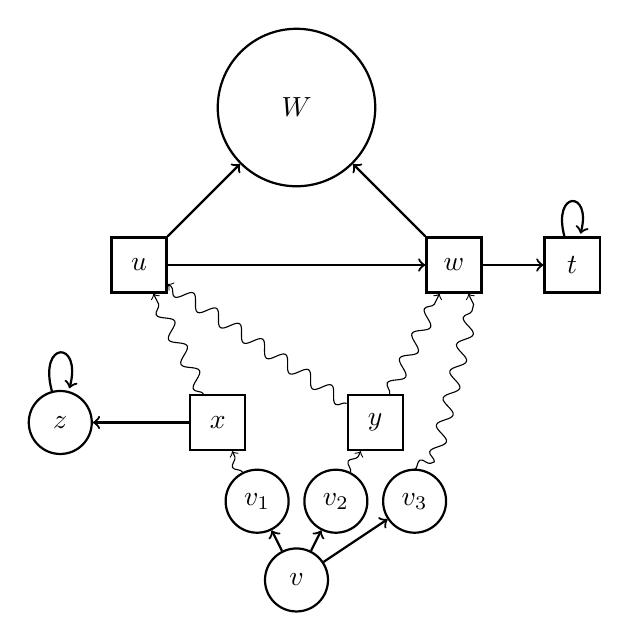
\begin{tikzpicture}
	\node at ( 0,-4) [player1] (1) {$v$};
	\node at ( -2,0) [player2] (2) {$u$};
	\node at ( 2,0) [player2] (3) {$w$};
	\node at ( 3.5,0) [player2] (8) {$t$};
	\node at ( -0.5,-3) [player1] (9) {$v_{1}$};
	\node at ( 0.5,-3) [player1] (10) {$v_{2}$};
	\node at ( 1.5,-3) [player1] (11) {$v_{3}$};
	\node at ( -1,-2) [player2] (4) {$x$};
	\node at ( 1,-2) [player2] (5) {$y$};
	\node at ( -3,-2) [player1] (6) {$z$};
	\node at ( 0,2) [otherLabel] (7) {$W$};
	
	\draw (2) edge (3);
	\draw (2) edge (7);
	\draw (3) edge (7);
	\draw (4) edge (6);
	\draw (3) edge (8);
	\draw (1) edge (9);
	\draw (1) edge (10);
	\draw (1) edge (11);
	\draw (6) edge[loop above] (6);
	\draw (8) edge[loop above] (8);
	\draw [->,snake=snake] (9) -- (4);
	\draw [->,snake=snake] (11) --  (1.5,-2.6) -- (1.75, -2.5) --  (2.25,-0.5) -- (3);
	\draw [->,snake=snake] (10) -- (5);
	\draw [->,snake=snake] (5) -- (2);
	\draw [->,snake=snake] (4) -- (2);
	\draw [->,snake=snake] (5) -- (3);
	\end{tikzpicture}
	\caption{Example demonstrating conditions}
	\label{figurelabel9}
\end{figure}

Figure~\ref{figurelabel9} explains the need for assigning ranks to
nodes in $V \backslash(W \cup \mathit{Front})$. \textit{Player~2} can prevent
\textit{Player~1} from entering $W$ forever by choosing the edge
$(x,z)$ at the potentially hazardous node $x$ while the potentially
hazardous node $y$ will always help \textit{Player~1} in reaching a
frontier node $u$ or $w$ depending on the outgoing edge \textit{Player
	2} chooses at $y$. These nodes are differentiated
while determining the admissible strategy for \textit{Player~1} at
$v$, hence $x$ is assigned the rank -1 and $y$ the rank
0.

Algorithm~\ref{alg:algorithm5} computes the set of
admissible strategies for reachability games. In step 1,
the winning set of nodes are computed $W$ for \textit{Player~1} using
Algorithm~\ref{alg:algorithm4}. Since any winning strategy of a
\textit{Player 1} winning node is \textit{admissible}, the rest of the
algorithm computes values of admissible strategies for the losing
nodes. In step 3, the set of frontier nodes are computed and stored
in $\mathit{Front}$. In steps 5-14, the ranks of the remaining nodes are computed
in $V \backslash W$. The loop terminates when all nodes in $V
\backslash(W \cup \mathit{Front})$ have been assigned a rank. In step 15, the set of all nodes are computed in $\mathit{Front}(v)$ for $v \in V_{1} \backslash
W$. In steps 17-30, the induced subgraph $G'$ is constructed for the
nodes in $\mathit{Front}(v)$, if $\mathit{Front}(v) \neq \emptyset$. In step 31, Algorithm~\ref{alg:algorithm6} is executed to compute the rank of
every vertex in the induced subgraph $G'$ and the remaining vertices
in $V \backslash W$. In step 34,
Algorithm~\ref{alg:algorithm7} is executed to compute the values of
admissible strategies for every component $C$ of the underlying
undirected graph of $G'$. In steps 40-42, the strategies for
\textit{Player~1} are returned.
\newline
\newline
Algorithm~\ref{alg:algorithm6} computes the rank for the nodes in $G'$. In steps 5 and 6, the nodes with out-degree 0 to 1 are initialized. In steps 9-12, ranks to the remaining nodes in $G'$ are assigned by checking if they have an outgoing edge to a node with the previously assigned rank. The value of rank at every iteration is incremented. The algorithm terminates when every node of $G'$ has been assigned a rank. 
\newline
\newline
Algorithm~\ref{alg:algorithm7} computes the values of admissible strategies at $v$ for component $C$  of the underlying undirected graph of $G'$. The following predicates are defined to describe the algorithm:
\begin{enumerate}
	\item $\mathrm{Lies}(v,v',P) \triangleq $ the edge $(v,v')$ lies on the path $P$ from $v$;
	\item $\mathrm{rAdmissible}(P,v,S,r) \triangleq $ $P$ is an r-admissible path from $v$ to a node in $S$ where all nodes in $S$ have rank $r$.
\end{enumerate}
The following sets are defined to describe the algorithm:
\begin{enumerate}
	\item $\mathrm{\mathit{PH}}(P) \triangleq $ the set of potentially hazardous nodes on the r-admissible path $P$;
	\item $\mathrm{Nodes}(P) \triangleq $ the set of nodes on an r-admissible path $P$ except the first and last one.
\end{enumerate}

Let $X$ be the set of all nodes $u$ in $C$, the present component of $G'$ whose rank is $r$, where $r$ is the current rank in the iteration. Let $h$ be the highest rank assigned to any node in $C$. The algorithm includes $v'$ in the set $A$ of values of admissible strategies at $v$ when one of the following conditions is satisfied, where the conditions are checked from top to bottom:
\begin{enumerate}
	\item $cond1 \triangleq \exists Q,r[r = h \: \wedge \: \mathrm{rAdmissible}(Q,v,X,r) \:  \wedge \: \mathrm{Lies}(v,v',Q) \: \wedge \: \mathrm{\mathit{PH}}(Q) = \emptyset]$
	%\smallskip
	\item $cond2 \triangleq \exists Q,r[r \neq h \: \wedge \: \mathrm{rAdmissible}(Q,v,X,r) \:  \wedge \: \mathrm{Lies}(v,v',Q) \: \wedge \: \mathrm{\mathit{PH}}(Q) \neq \emptyset \newline
	\wedge \forall w \in \mathrm{Nodes}(Q)[rank(w) = 0 \: \vee \: r \leq rank(w) \leq h] ]$
	%\smallskip
	\item $cond3 \triangleq \exists Q,r[r \neq h \: \wedge \: \mathrm{rAdmissible}(Q,v,X,r) \: \wedge \: \mathrm{Lies}(v,v',Q) \: \wedge \: \mathrm{\mathit{PH}}(Q) = \emptyset]$  
	%\smallskip
	\item $cond4 \triangleq \exists Q,r[\mathrm{rAdmissible}(Q,v,X,r) \: \wedge \: \mathrm{Lies}(v,v',Q) \: \wedge \: \mathrm{\mathit{PH}}(Q) \neq \emptyset]$
\end{enumerate}

Figure~\ref{figurelabel9} explains the need for conditions $cond1$ to
$cond4$. The r-admissible path $(v--x--u)$ illustrates the use for
$cond4$ due to the edge $(x,z)$ which results in $x$ having rank
-1. Further, the r-admissible paths $(v--y--u)$ and $(v--y--w)$ show
the use for $cond2$ due to the nature of $y$ whereas the path
$(v--w)$ shows the use for $cond3$ as the path does not have any
potentially hazardous node. Since $cond1$ is not satisfied (which is
the same as $cond3$ except the path should be from $v$ to $u$ instead
of $w$), the \textit{Player~1} strategy $\sigma_{1}$ that chooses
$(v,v_{1})$ that lies on the r-admissible path $(v--x--u)$ is no
better than the \textit{Player~1} strategy $\sigma_{2}$ that chooses
$(v,v_{2})$ that lies on any of the two r-admissible paths
$(v--y--u)$ or $(v--y--w)$ against any \textit{Player~2} strategy. On
the other hand, the \textit{Player~1} strategy $\sigma_{2}$ that
chooses $(v,v_{2})$ performs better than the \textit{Player~1}
strategy $\sigma_{3}$ that chooses $(v,v_{3})$ that lies on the
r-admissible path $(v--w)$ against the \textit{Player~2} strategy
\{$u \mapsto k\in W, w \mapsto t, t \mapsto t$\}. Hence $\sigma_{1}$
and $\sigma_{2}$ are admissible strategies and not $\sigma_{3}$. The
algorithm iterates from the highest rank to the lowest rank in
$C$. For each rank $r$, it checks from conditions $cond1$ to $cond4$
in order. Whenever a condition from $cond1$ to $cond3$ is satisfied,
it returns the set $A$. If $cond4$ is satisfied, the algorithm
proceeds to the next lower rank after storing the set $A$ of possible
values of admissible strategies at node $v \in V_{1} \backslash W$.
\begin{algorithm}
	\caption{Admissible Strategies for Reachability Games}
	\textbf{Input} Game structure $G := (V,E)$ and $R \subseteq V$ \\ 
	\textbf{Output} Set of admissible strategies for \textit{Player~1}
	\label{alg:algorithm5}
	\begin{algorithmic}[1]
		\STATE Compute $W$ for \textit{Player~1} using Algorithm~\ref{alg:algorithm4}
		\STATE $G' := null$
		\STATE $\mathit{Front} := \{ v | v \in V_{2} \backslash W \: and  \: \exists u . (v,u) \in W\}$
		\FOR{every $v \in V_{1} \backslash W$}
		\FOR{every node $u \in V_{1} \backslash W \cup V_{2} \backslash (W \cup \mathit{Front} \cup \mathit{PH})$}
		\STATE $rank(u) := 0$
		\ENDFOR
		\FOR{every node $v \in \mathit{PH}$}
		\IF{$v$ is the source of an infinite path that does not contain a node in $\mathit{Front}$}
		\STATE $rank(v) := -1$
		\ELSE
		\STATE $rank(v) := r$, where $r$ is the lowest ranked node in $\mathit{Front}$ to which it has an r-admissible path
		\ENDIF
		\ENDFOR
		\STATE Let $\mathit{Front}(v)$ be the set containing all $u \in \mathit{Front}$ such that $\mathit{FPaths}(v,u) \neq \emptyset$. 
		\IF{$\mathit{Front}(v) \neq \emptyset$} 
		\STATE $G' = (V',E') := (\emptyset,\emptyset)$
		\FOR{every vertex $p \in \mathit{Front}(v)$}
		\STATE $V' := V' \cup \{p\}$
		\ENDFOR
		\FOR{every pair of nodes $p_{1},p_{2} \in \mathit{Front}(v)$} 
		\IF{all paths from $p_{1}$ lead to $p_{2}$ in $G \backslash W$ such that no node in $\mathit{Front}$ repeat itself and do not contain a node $u$ with $rank(u) = -1$}
		\IF{$(p_{2},p_{1}) \in E'$}
		\STATE $E' := E' \backslash \{(p_{2},p_{1})\}$
		\ELSE
		\STATE $E' := E' \cup \{(p_{1},p_{2})\}$
		\ENDIF
		\STATE Goto step 11.
		\ENDIF
		\ENDFOR
		\STATE Call Algorithm~\ref{alg:algorithm6} to compute the rank of nodes in $G'$
		\algstore{algorithm5}
\end{algorithmic}
\end{algorithm}

\begin{algorithm}
\begin{algorithmic}[1]
\algrestore{algorithm5} 
		\STATE $S(v) := \emptyset$ \COMMENT{$S$ is the set of all $v'$ s.t. $\sigma(v) = v'$ for some admissible strategy $\sigma$}
		\FOR{every component $C$ in the underlying undirected graph of $G'$}
		\STATE Execute Algorithm~\ref{alg:algorithm7} for $C$
		\STATE $S(v) := S(v) \cup A$
		\ENDFOR
		\STATE Re-initialize $G' = (V',E')$ with $V' := \emptyset$, $E' := \emptyset$
		%\ENDFOR
		\ENDIF
		\ENDFOR
		\STATE At any \textit{Player~1} node $v \in W$, play according to any winning strategy
		\STATE At any \textit{Player~1} node $v \notin W$ such that $\mathit{Front}(v) = \emptyset$, choose an arbitrary move
		\STATE At any other \textit{Player~1} node $v$, choose any node in $S(v)$
	\end{algorithmic}
\end{algorithm}

\begin{algorithm}
	\caption{Compute rank for nodes in $G'$}
	\label{alg:algorithm6}
	\begin{algorithmic}[1]
		\FOR{every component $C$ of the underlying undirected graph of $G'$}
		\STATE $r := 1$
		\WHILE{$C$ has vertices left to be assigned a rank}
		\IF{$r = 1$}
		\FOR{every vertex $v$ in $G'$ with out-degree 0}
		\STATE $rank(v) := r$
		\ENDFOR
		\ELSE
		\FOR{every vertex $v$ in $G'$ that does not have a rank and has an edge to $v'$ where $rank(v') = r - 1$}
		\STATE $rank(v) := r$
		\ENDFOR
		\ENDIF
		\STATE $r := r + 1$
		\ENDWHILE
		\ENDFOR
	\end{algorithmic}
\end{algorithm}

\begin{algorithm}
	\caption{Values of admissible strategies at $v$ for component $C$}
	\textbf{Output} $ A = \{v' \, | \, \sigma(v) = v'$ for an admissible strategy at $v\}$  
	\label{alg:algorithm7}
	\begin{algorithmic}[1]
		\STATE $A := \emptyset$
		\STATE $h := $ highest rank in $C$
		\STATE $l := $ lowest rank in $C$            
		\FOR{$r := h$ to $l$}
		\STATE $flag := 0$
		\STATE $flag1 := 0$
		\STATE $X := $ set of all nodes in $C$ with rank $r$
		\STATE Determine the set $A'$ of all $v'$ s.t. $(v,v')$ lies on an r-admissible path $Q$ from $v$ to a node $u \in X$ where $rank(w) = 0$ for every $w \in \mathrm{Nodes}(Q)$ 
		\STATE $A := A \cup A'$ \COMMENT{Condition $cond1$ holds. $Q$ does not contain any node in $\mathit{PH}$}
		\IF{$A' \neq \emptyset$}
		\STATE $flag := 1$
		\ENDIF
		\IF{$r = h$ and $flag = 1$}      
		\STATE return $A$   \COMMENT{$A' \neq \emptyset$}
		\ENDIF
		\STATE Determine the set $A'$ of all $v'$ s.t. $(v,v')$ lies on an r-admissible path $Q$ from $v$ to a node in $X$      \COMMENT{$Q$ contains at least one node in $\mathit{PH}$}
		\IF{$r = h$}
		\STATE $A := A \cup A'$ \COMMENT{Condition $cond2$ holds}
		\ELSE
		\IF{$A' = \emptyset$} 
		\STATE return $A$ \COMMENT{$r \neq h$}
		\ELSE 
		\FOR{every $v' \in A'$}
		\STATE $\mathbb{Q} := $ the set of all r-admissible paths that have the edge $(v,v')$
		\FOR{every $Q \in \mathbb{Q}$}
		\IF{$w \in \mathrm{Nodes}(Q)$ s.t. $rank(w) = -1$ or $1 \leq rank(w) < r$}
		\STATE $flag1 := 1$
		\STATE break
		\ENDIF
		\ENDFOR
		\IF{$flag1 = 0$}
		\STATE $A := A \backslash \{ v | v \in A'$ in step 8\} \COMMENT{Condition $cond3$ holds}
		\STATE return $A$
		\ENDIF
		\ENDFOR
		\algstore{algorithm7}
  \end{algorithmic}
\end{algorithm}

\begin{algorithm}
\begin{algorithmic}[1]
\algrestore{algorithm7}
		\IF{$flag = 1$}
		\STATE return $A$
		\ELSE
		\STATE $A := A \cup A'$ from step 16
		\ENDIF
		\ENDIF
		\ENDIF
		\ENDFOR
	\end{algorithmic}
\end{algorithm}

The following results are needed to prove the correctness of
Algorithm~\ref{alg:algorithm5}
(Corollary~\ref{corollary2}). 
Lemma~\ref{lemma2} states that any
admissible strategy would choose an edge along an r-admissible path
from any node $v \in V_{1} \backslash W$ from which $W$ is
reachable. 
Lemma~\ref{lemma3} states that if any of the conditions
$cond1$ or $cond2$ or $cond3$ is satisfied for an r-admissible path
which terminates at a node in $\mathit{Front}$ with rank $r$, then no
strategy that chooses an edge along an r-admissible path which
terminates at a node in $\mathit{Front}$ with rank $k < r$ is
admissible. 
Lemma~\ref{lemma4} states that if there is an r-admissible path $P$ which 
terminates at a node in $\mathit{Front}$ with rank $k$ and there is an
admissible strategy that chooses an edge along an
r-admissible path which terminates at a node in $\mathit{Front}$
with rank $r<k$, then $P$ must satisfy only condition $cond4$ and not 
any of $cond1$ or $cond2$ or $cond3$.
Theorem~\ref{theorem2} states that a strategy is
admissible iff at least one of the conditions $cond1,\ldots,cond4$
holds when they are checked in that order.

\begin{lemma}
	\label{lemma2}
	If $\sigma$ is an admissible \textit{Player~1} strategy, $v \in V_{1} \backslash W$ and the set $W$ is reachable from $v$ in $G$, then $\sigma(v) = v'$ implies the pair $(v,v')$ satisfies $\exists Q,r[\mathrm{rAdmissible}(Q,v,X,r) \:  \wedge \: \mathrm{Lies}(v,v',Q)]$.
\end{lemma}
\begin{proof}
	If $v \in V_{1} \backslash W$ and $W$ is reachable from $v$ then there is always an r-admissible path from $v$ by considering only the paths that end in the first node in $\mathit{Front}$ and choosing those among them that contain a minimal number of \textit{Player~2} nodes. An admissible strategy $\sigma$ would always choose a successor node $v'$ at $v$ where $v'$ lies on an r-admissible path because such a path contains a minimal set of \textit{Player~2} nodes that can take the game away from $W$. The proof is along similar lines as Theorem~\ref{theorem1} for safety. 
\end{proof}

\begin{lemma}
	\label{lemma3}
	If $\sigma$ is an admissible strategy with $\sigma(v) = v'$ where $(v,v')$ lies on an r-admissible path $Q$ satisfying the following properties:
	\begin{enumerate}
		\item $Q$ terminates at a node in $\mathit{Front}(v)$ with rank $r$ and,
		\item no node in $Q$ has rank -1
	\end{enumerate}
	then, for any other strategy $\sigma'$ with $\sigma'(v) = v''$ where $(v,v'')$ lies on an r-admissible path $Q'$ that terminates at a node in $\mathit{Front}(v)$ with rank $k > r$, the relation $val(\sigma,\rho,v) > val(\sigma',\rho,v)$ holds for all \textit{Player~2} strategies $\rho$.
\end{lemma}
\begin{proof}
	It is observed that if no node $u$ along the r-admissible path $Q$ has $rank(u) = -1$, then the path $Q$ will inevitably reach a node in $\mathit{Front}(v)$ with rank $k \geq 1$ as only the nodes ranked as -1 have the potential to prevent the game from reaching $\mathit{Front}(v)$ forever. 
	Further, it is clear from the computation of rank that for any two nodes $u,w \in \mathit{Front}(v)$ and in the same component of the underlying undirected graph of $G'$ where $rank(u) > rank(w)$, there does not exist any path from $w$ to $u$ and all paths from $u$ lead to $w$ in $G \backslash W$ and do not include any potentially hazardous node $u'$ with $rank(u') = -1$.
	
	From the observations the following cases are to be considered:
	
	\textit{Case 1}: $Q'$ has at least one node $u$ where $rank(u) = -1$
	\newline This implies that a node in $\mathit{Front}(v)$ with rank $k$ may not be reached at all, whereas by following strategy $\sigma$, one can definitely reach $\mathit{Front}(v)$ and enter $W$ through one of the nodes $w \in \mathit{Front}(v)$, with $rank(w) \in [r,h]$. Hence $val(\sigma,\rho,v) > val(\sigma',\rho,v)$ in this case.
	
	\textit{Case 2}: $Q'$ has no node $u$ where $rank(u) = -1$
	\newline This implies that the path $Q$ will inevitably reach a node
	in $\mathit{Front}(v)$ with rank $k \geq 1$. So, by following
	strategy $\sigma$, one can definitely reach $\mathit{Front}(v)$ and
	enter $W$ through one of the nodes $w \in \mathit{Front}(v)$, with
	$rank(w) \in [r,h]$ and by following strategy $\sigma'$, $W$ can be entered through one of the nodes $w \in \mathit{Front}(v)$, with $rank(w)
	\in [k,h]$ as shown in Figure~\ref{figurelabel4}. Since $k < r$, if
	at one of the nodes $u' \in \mathit{Front}(v)$ with $k < rank(u') <=
	r$ \textit{Player~2} chooses the edge that leads to $W$ and at none
	of the nodes with rank in $[k,h]$ \textit{Player~2} choose the edge
	that leads to $W$, then $Out(\sigma,\rho,v) \in \mathit{Win}$ but
	$Out(\sigma',\rho,v) \notin \mathit{Win}$. Hence $val(\sigma,\rho,v)
	> val(\sigma',\rho,v)$ in this case as well.
	\begin{figure}[thpb]
		\centering
		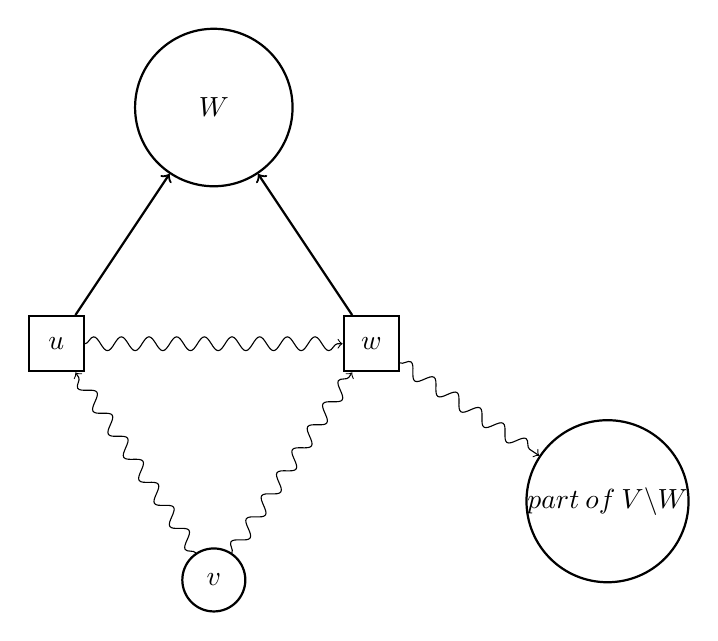
\begin{tikzpicture}
		\node at ( 0,0) [player1] (1) {$v$};
		\node at ( -2,3) [player2] (2) {$u$};
		\node at ( 2,3) [player2] (3) {$w$};
		\node at ( 0,6) [otherLabel] (4) {$W$};
		\node at ( 5,1) [otherLabel] (5) {$ part\:of\: V \backslash W$};
		\draw (2) edge (4);
		\draw (3) edge (4);
		\draw [->,snake=snake] (1) -- (2);
		\draw [->,snake=snake] (1) -- (3);
		\draw [->,snake=snake] (2) -- (3);
		\draw [->,snake=snake] (3) -- (5);
		\end{tikzpicture}
		\caption{Player~1 chooses edge leading to $u$ over edge leading to $v$}
		\label{figurelabel4}
	\end{figure}
\end{proof}

\begin{lemma}
	\label{lemma4}
	\begin{enumerate}
		\item Suppose $\sigma$ is an admissible strategy with $\sigma(v) = v'$ and $(v,v')$ lies on an r-admissible path leading to a node in $\mathit{Front}(v)$ with rank $r \neq h$. Then for all admissible strategies $\sigma'$ with $\sigma'(v) = v''$ where $v' \neq v''$ if the pair $(v,v'')$ lies on an r-admissible path leading to a node in $\mathit{Front}(v)$ with rank $k$, where $r+1 \leq k \leq h$ then the pair $(v,v'')$ satisfies only $cond4$ among the four conditions on page 22-23.
		\item Suppose $\sigma'$ is an admissible strategy with $\sigma'(v) = v''$ and the pair $(v,v'')$ lies on an r-admissible path leading to a node in $\mathit{Front}(v)$ with rank $k$, where $r+1 \leq k \leq h$, for some $r$ and further satisfies only $cond4$ among the four conditions on page 22-23. Further suppose there is a $v'$ with $v' \neq v''$ and $(v,v')$ lies on an r-admissible path leading to a node in $\mathit{Front}(v)$ with rank $r$. Then there exists an admissible strategy $\sigma$ satisfying $\sigma(v) = v'$. 
	\end{enumerate}
\end{lemma}
\begin{proof}
	\textit{(1)}: For the sake of contradiction assume that $\sigma$ is an admissible strategy and for an admissible strategies $\sigma'$ with $\sigma'(v) = v''$ where $v' \neq v''$ the pair $(v,v'')$ lies on an r-admissible path $Q$ leading to a node in $\mathit{Front}(v)$ with rank $k$, where $r+1 \leq k \leq h$ and satisfies $cond1$, $cond2$ or $cond3$. If $cond1$ or $cond3$ is satisfied, then there are no potentially hazardous nodes along the r-admissible path $Q$. So a node in $\mathit{Front}(v)$ with rank $k > r$ will definitely be reached along all paths starting with the pair $(v,v'')$. From Lemma~\ref{lemma3}, $val(\sigma',\rho,v) > val(\sigma,\rho,v)$ for any \textit{Player~2} strategy $\rho$. This implies that $Out(\sigma',\rho,v) \in \mathit{Win}$ but $Out(\sigma,\rho,v) \notin \mathit{Win}$, a contradiction. If $cond2$ is satisfied, then all \textit{Player~2} nodes along the r-admissible path $Q$ have rank $r' \in [r+1,h]$. So a node in $\mathit{Front}(v)$ with rank $k > r$ will definitely be reached along all paths starting with the pair $(v,v'')$. From Lemma~\ref{lemma3}, $val(\sigma',\rho,v) > val(\sigma,\rho,v)$ for any \textit{Player~2} strategy $\rho$. This implies that $Out(\sigma',\rho,v) \in \mathit{Win}$ but $Out(\sigma,\rho,v) \notin \mathit{Win}$, again a contradiction.
	
	\textit{(2)}: For the sake of contradiction assume that for
	all admissible strategies $\sigma'$ with $\sigma'(v) = v''$ the pair
	$(v,v'')$ lies on an r-admissible path leading to a node in $\mathit{Front}(v)$
	with rank $k$, where $r+1 \leq k \leq h$, for some $r$ and satisfies
	only $cond4$. Further, assume there is a $v'$ with $v' \neq v''$ and
	$(v,v')$ lies on an r-admissible path leading to a node in $\mathit{Front}(v)$
	with rank $r$, and there does not exist an admissible strategy
	$\sigma$ satisfying $\sigma(v) = v'$. If only $cond4$ is satisfied
	for the pair $(v,v'')$, then there is at least one potentially
	hazardous node $u$ with $rank(u) = -1$ in the r-admissible path
	$Q$. From Lemma~\ref{lemma3}, there is no guarantee that a node in
	$\mathit{Front}(v)$ with rank $k > r$ will be reached. Hence it cannot be said that $val(\sigma',\rho,v) > val(\sigma,\rho,v)$ for any
	\textit{Player~2} strategy $\rho$, thus arriving at a
	contradiction. Hence both $\sigma$ and $\sigma'$ are admissible. 
\end{proof}

\begin{theorem}
	\label{theorem2}
	The following statements are equivalent:
	\begin{enumerate}
		\item $\sigma$(v) = v' for an admissible \textit{Player~1} strategy $\sigma$ where $v \in V_{1} \backslash W$ and $W$ is reachable from $v$ in $G$
		\item the pair $(v,v')$ satisfies one of the following statements where $1 \leq r \leq h$:
		\begin{enumerate}
			\item $cond1$
			\item $\sim cond1 \Rightarrow cond2$
			\item $\sim(cond1 \vee cond2) \Rightarrow cond3$
			\item $\sim(cond1 \vee cond2 \vee cond3) \Rightarrow cond4$.
		\end{enumerate}
	\end{enumerate}
\end{theorem}
\begin{proof}
	$\mathit{1} \Rightarrow \mathit{2}$
	\newline By Lemma~\ref{lemma2} $(v,v')$ lies on an r-admissible path $Q$ from $v$ to $u \in \mathit{Front}(v)$. Let $u$ be of rank $r$.
	\newline \textit{Case 1: r = h}
	\newline For the sake of contradiction assume that none of the above four statements is true. For this to hold, all the conditions $cond1$ to $cond4$ are required to be false. Since $r = h$, $cond2$ and $cond3$ are false. Since $cond1$ is false and $\sigma$ is an admissible strategy, it can be concluded that $\mathrm{\mathit{PH}}(Q) \neq \emptyset$. Since statement (d) and therefore $cond4$ is false, by Lemma~\ref{lemma2} $\mathrm{\mathit{PH}}(Q) = \emptyset$ for all r-admissible paths $Q$, which is a contradiction.  
	\newline \textit{Case 2: $r \neq h$}
	\newline Again for the sake of contradiction assume that none of the above four statements is true. Since $r \neq h$, $cond1$ is false. Since, Lemma~\ref{lemma4} holds for all admissible strategies $\sigma'$ with $\sigma'(v) = v''$ and $v'' \neq v'$, the pair $(v,v'')$ lies on an r-admissible path leading to a node in $\mathit{Front}(v)$ with rank $k$, where $r+1 \leq k \leq h$, for some $r$ and satisfies only $cond4$ among the four conditions on page 22-23. Since by assumption statement (b) is false, $cond2$ is false. Since $\sigma$ is an admissible strategy, it can be concluded that either of the following two properties must hold for $Q$:
	\begin{enumerate}
		\item $\mathrm{\mathit{PH}}(Q) = \emptyset$
		\item $\exists w \in \mathrm{Nodes}(Q)[1 \leq rank(w) < r]$.
	\end{enumerate}
	Since by assumption, $cond3$ is also false, and $\sigma$ is an admissible strategy, it can be concluded that $\mathit{PH}(Q) \neq \emptyset$. This implies property 2 must hold and property 1 must not for $cond2$ and $cond3$ to be false at the same time. Since statement (d) and therefore $cond4$ is false, by Lemma~\ref{lemma2} $\mathrm{\mathit{PH}}(Q) = \emptyset$ for all r-admissible paths $Q$, which is a contradiction.
	\newline $\mathit{2} \Rightarrow \mathit{1}$
	\newline For the sake of contradiction assume that one of the four statements is true and $\sigma(v) \neq v'$ for all admissible strategies $\sigma$. If statement (a) is true and therefore $cond1$ is true, from the first observation in the proof of Lemma~\ref{lemma3} any r-admissible path starting with the pair $(v,v')$ will inevitably reach a node in $\mathit{Front}(v)$. Hence $\sigma$ is admissible which is a contradiction. If statement (b) is true and statement (a) is false, then $cond1$ is false and $cond2$ is true, from the first observation in the proof of Lemma~\ref{lemma3} any r-admissible path starting with the pair $(v,v')$ will inevitably reach a node in $\mathit{Front}(v)$. Hence $\sigma$ is admissible, a contradiction. If statement (c) is true and statements (a) and (b) are false, then $cond1$ and $cond2$ are false and $cond3$ is true. Since $cond3$ is true, from the first observation in the proof of Lemma~\ref{lemma3} any r-admissible path starting with the pair $(v,v')$ will inevitably reach a node in $\mathit{Front}(v)$. Hence $\sigma$ is admissible, a contradiction. If statement (d) is true and statements (a), (b) and (c) are false, then only $cond4$ is true. If $r = h$ and conditions $cond1$ to $cond3$ are false, $\sigma$ is admissible. Otherwise, from Lemma~\ref{lemma4} it is known that for all admissible strategies $\sigma'$ with $\sigma'(v) = v''$, the pair $(v,v'')$ lies on an r-admissible path leading to a node in $\mathit{Front}(v)$ with rank $k$, where $r+1 \leq k \leq h$, for some $r$ and satisfies only $cond4$. Hence $\sigma$ is admissible, which is again a contradiction. 
\end{proof}

The following result about the correctness of Algorithm~\ref{alg:algorithm5} is a consequence of Theorem~\ref{theorem2}.

\begin{corollary}
	\label{corollary2}
	Algorithm~\ref{alg:algorithm5} returns all the admissible strategies for a reachability game.
\end{corollary}

\section{Complexity}
The time complexity of Algorithm~\ref{alg:algorithm4} is $O(|V| +
|E|)$. Step 3 of Algorithm~\ref{alg:algorithm5} takes $O(|V| + |E|)$
time. In step 5, computing the set of all paths takes
$O((|V|+|E|)*(|P|+1))$ time~\cite{ElementaryCircuits}, where $|P|$ is
the number of paths. In steps 16 through 30, to determine an edge from
$p_{1}$ to $p_{2}$ for $p_{1}, p_{2} \in V'$, all paths need to be checked from $p_{1}$ to $p_{2}$ which takes $O(|P|^{2})$
time. Algorithm~\ref{alg:algorithm6} requires $O(|\mathit{Front}(v)|)$
time to compute the rank of a vertex. Algorithm~\ref{alg:algorithm7}
runs for every component $C$ in $G'$. The computation of
Algorithm~\ref{alg:algorithm7} takes $O(|P|^{2})$ time. Hence the
overall complexity of Algorithm~\ref{alg:algorithm5} is $O(|V| + |E| +
|V_{1} \backslash W|*((|V|+|E|)*(|P|+1) + |P|^{2} +
|\mathit{Front}(v)| + |C|*|P|^{2}))$, where $|C|$ denotes the number
of components in $G'$ for $v \in V_{1} \backslash W$. This is
$O(|V|!)$, \ie, $O(2^{|V|log|V|})$.
%%%%%%%%%%%%%%%%%%%%%%%%%%%%%%%%%%%%%%%%%%%%%%%%%%%%%%%%%%%%%%%%%%%%%%%%%%%%%%%%
%2345678901234567890123456789012345678901234567890123456789012345678901234567890
%        1         2         3         4         5         6         7         8
% THESIS CONCLUSIONS
\def\baselinestretch{1}
\chapter{Conclusions}
\label{chap:conclusions}
\ifpdf
    \graphicspath{{Conclusions/Figures/PNG/}{Conclusions/Figures/PDF/}{Conclusions/Figures/}}
\else
    \graphicspath{{Conclusions/Figures/EPS/}{Conclusions/Figures/}}
\fi
\def\baselinestretch{1.0}

% quote


The work aims to solve admissible strategies for safety and
reachability objectives which are arguably the most important among all non-prefix-independent goals. The work uses graph-theoretic notions to provide a solution for the problem at hand. 

The work is a special case of~\cite{PerimeterOfWorldModel,CompositionalSynthesis}
where only two properties are taken into consideration and much simpler algorithms are proposed for them which are also lower in complexity (precisely $O(2^{|V|log|V|})$ time) than the double exponential algorithm in~\cite{PerimeterOfWorldModel,CompositionalSynthesis}.

The algorithms have been proven to be correct and exhaustive. Previous claims  made by Faella~\cite{AdmissibleInfiniteGames} have also shown to be incorrect. Work on cooperation and rational behavior of players is now an emergent area of research~\cite{AssumptionSynthesis,PerimeterOfWorldModel,CompositionalSynthesis,AdmissibleInfiniteGames,RationalSynthesis} and the work done claims to be the first approach in solving zero sum games with winning conditions as safety and reachability in exponential time with graph-theoretic notions. The work can be extended to solve objectives like \textit{B$\ddot{u}chi$}, \textit{Muller}, \textit{Parity}, etc. in future. The work is also useful in compositional synthesis where each component is to be composed and admissible strategies are to be determined and shown to hold good.

%\appendix
%%%%%%%%%%%%%%%%%%%%%%%%%%%%%%%%%%%%%%%%%%%%%%%%%%%%%%%%%%%%%%%%%%%%%%%%%%%%%%%%%
%2345678901234567890123456789012345678901234567890123456789012345678901234567890
%        1         2         3         4         5         6         7         8
% THESIS APPENDIX

\chapter{Gesture Vocabulary} 
\label{chap:appendixA}


\begin{figure}
    \centering
    \includegraphics[width=0.8\textwidth]{Chapter4/Figures/Figures/gv.PNG}
    \caption{Proposed gesture vocabulary}
    \label{fig:gs}
\end{figure}


%\chapter{Survey}
\label{chap:appendixB}


%\begin{figure}
%\setboolean{@twoside}{false}
% Uncomment the follow line to show the survey
\includepdf[pages=1-,scale=0.8,pagecommand={}]{Appendix2/gbhri3_format.pdf}
%\end{figure}

%\begin{figure}
 %\centering 
 %\includegraphics{Appendix2/gbhri3_format.pdf}
%\end{figure}
%\bibliographystyle{Classes/RoboticsBiblio}    % bibliography style
\bibliographystyle{ieeetr}
\renewcommand{\bibname}{References}           % change default name Bibliography to References
\bibliography{References/references}          % References file
\addcontentsline{toc}{chapter}{References}    % add References to contents page
%\addcontentsline{toc}{section}{References}
\nocite{*}
\end{document}
